 \documentclass[conference]{IEEEtran}
\IEEEoverridecommandlockouts
%\usepackage{hyphenat}
\usepackage[ruled,vlined]{algorithm2e}
\usepackage{amsmath}
\usepackage{xspace}
\usepackage[binary-units=true]{siunitx}
\usepackage{ulem}
%\usepackage{censor}
\usepackage[table]{xcolor}
\usepackage{graphicx}
\usepackage{hyperref}
\usepackage{tabularx}

\usepackage{subcaption}
\usepackage{booktabs}
\usepackage{multirow}
\usepackage{listings}

\hypersetup{
    colorlinks=true,
    linkcolor=black,
    citecolor=blue,
    filecolor=black,
    urlcolor=blue}

\def\BibTeX{{\rm B\kern-.05em{\sc i\kern-.025em b}\kern-.08em
    T\kern-.1667em\lower.7ex\hbox{E}\kern-.125emX}}
    
\begin{document}

\newcommand{\fslspm}{FSL-SPM\xspace}
\newcommand{\fslafni}{FSL-AFNI\xspace}
\newcommand{\afnispm}{AFNI-SPM\xspace}


\title{Comparing tool variability and numerical variability in fMRI analyses}

\author{Ali Salari$^1$, Other Authors$^1$, Tristan Glatard$^1$ \\ 
$^1$ Department of Computer-Science and Software Engineering, Concordia University, Montreal, Canada}

\maketitle
\begin{abstract}
  
\end{abstract}

\begin{IEEEkeywords}
\end{IEEEkeywords}


\section{Introduction}

\begin{itemize}
    \item We presented a framework that can investigate the numerical instability of the pipelines based on Monte-Carlo arithmetic
    by creating a Fuzzy environment, so that instrument mathematical functions implemented in mathematical system libraries (libmath). 

    \item Methodological choice can influence the final determining areas of brain activation.
    This opens so results flexibility~\cite{bowring2019exploring,bowring2021isolating}. 
  
    \item In this paper, we aim to answer the questions 1) how the fMRI analyses are numerically stable?
    2) how the numerical variability is in comparison with the tool variability?
\end{itemize}

\section{Materials and Methods}

\subsection{Fuzzy libmath environment}

To simulate the machine level uncertainty, we used the method introduced in~\cite{salari2021accurate} called Fuzzy libmath (FL).
FL uses Monte Carlo Arithmetic (MCA) to introduce a controlled amounts of noise in the floating-point operations,
which models floating-point rounding and catasrophic cancellation errors.
This is automated using Verificarlo tool~\cite{denis2015verificarlo} that implements MCA in the compilation time.
The perturbation is introduced in a given number of least-significant bits so that
the number of bits in the mantissa that will not be perturbed is defined as the virtual precision.​

% MCA models floating-point roundoff and cancellations errors through random
% perturbations, allowing for the estimation of error distributions from
% independent random result samples. MCA simulates computations at a given
% \emph{virtual precision} using the following perturbation:
% \begin{equation} \label{eq:mca_inexact}
%   inexact(x) = x + 2^{e_x-t}\xi
%   \label{mcadefinition}
% \end{equation}
% where $e_x$ is the exponent in the floating-point representation of $x$,
% $t$ is the virtual precision and $\xi$ is a random uniform variable of
% $(-\frac{1}{2}, \frac{1}{2})$.

% MCA allows for three perturbation modes: Random Rounding (RR) introduces the
% perturbation in function outputs, simulating roundoff errors; Precision Bounding
% (PB) introduces the perturbation in function operands, allowing for the
% detection of catastrophic cancellations; and, Full MCA combines RR and PB,
% resulting in the following perturbation:
% \begin{equation} \label{eq:mca_modes}
%   mca\_mode(x \circ y) = inexact_{RR}(  inexact_{PB}(x) \circ inexact_{PB}(y) )
% \end{equation}

% We instrumented the GNU mathematical library with MCA using
% Verificarlo~\cite{denis2015verificarlo}, a tool that (1) uses the Clang
% compiler to generate an LLVM (\url{http://llvm.org}) Intermediate
% Representation (IR) of the source code, (2) replaces floating-point operations
% in the IR by a call to the Verificarlo API, and (3) compiles the modified IR to
% an executable using LLVM. The perturbation applied by the Verificarlo API
% can be configured at runtime, for instance to change the virtual
% precision applied to single- and double-precision floating-point values.

In this framework, mathematical functions embeded in the operating system GNU mathematical library (libmath)
are targeted to be instrumented.
It instrument the functions by wrapping them so that only the output of the original functions be perturbed
instead of input or their implementation.
This is achieved by adding a floating-point zero to the output of the original function which results into perturbations.
Listing~\ref{algo:wrapper} shows an example of this wrapping for the log function in both single and double precisions.
This functionality helps to avoid of some issues in deterministic arithmetics like producing results out of the function definition.


% To simulate OS updates, we introduce random perturbations in the GNU
% mathematical library, the main mathematical library in GNU/Linux systems.
% Instrumenting mathematical libraries with MCA raises a number of issues as
% many functions assume deterministic arithmetic. For instance, applying random
% perturbations around a discontinuity or within piecewise approximations
% results in large variations and a total loss of significance that are not
% relevant in our context. Therefore, we have applied MCA to proxy
% mathematical functions wrapping those in the original library, such that only
% the outputs of the original functions were perturbed but not their inputs or
% the implementations themselves. This technique allows us to control the
% magnitude of the perturbation as perceived by the application.


The instrumented math functions so called ``fuzzy libmath", is loaded in the pipeline using LD\_PRELOAD, a Linux mechanism
to force load a shared library into an executable. ​
As a result, functions defined in fuzzy libmath transparently overload the original ones without the need to modify or
recompile the analysis pipeline.​
Also, this technique allows measuring the effect of numerical noise by running a program multiple times.​
It is important to review the software dependencies of the pipelines to be sure that are involved with the same library that
we arep erturbing.

% The resulting MCA-instrumented mathematical library, ``fuzzy libmath" (FL), is
% loaded in the pipeline using \texttt{LD\_PRELOAD}, a Linux mechanism to
% force-load a shared library into an executable. As a result, functions defined in fuzzy libmath
% transparently overload the original ones without the need to modify
% or recompile the analysis pipeline. Fuzzy libmath functions call the original
% functions through \texttt{dlsym}, a function that returns the memory address of
% a symbol. To trigger MCA instrumentation, a floating-point zero is added to the
% output of the original function and the result of this sum is perturbed and
% returned.

% \begin{description}
%   \item[$\bullet$ ] libmath Fuzzy allows you to study the numerical stability of tools and pipelines. 
%   \item[$\bullet$ ] It is based on MCA perturbations so that applies slight noise on floating-point operations.
%   \item[$\bullet$ ] It does not need source code modification or recompilation, and simply works using the Linux LD\_PRELOAD environment variable.
%   \item[$\bullet$ ] The library call interposition technique enables us to assess the tools that are dynamically linked to the mathematical library.
% \end{description} 


% \lstdefinestyle{customc}{
%   belowcaptionskip=1\baselineskip,
%   breaklines=true,
%   frame=L,
%   xleftmargin=\parindent,
%   language=C,
%   showstringspaces=false,
%   basicstyle=\footnotesize\ttfamily,
%   keywordstyle=\bfseries\color{green!40!black},
%   commentstyle=\itshape\color{purple!40!black},
%   identifierstyle=\color{blue},
%   stringstyle=\color{orange},
% }

\lstdefinestyle{customasm}{
  belowcaptionskip=1\baselineskip,
  frame=L,
  xleftmargin=\parindent,
  language=[x86masm]Assembler,
  basicstyle=\footnotesize\ttfamily,
  commentstyle=\itshape\color{purple!40!black},
}
\lstinputlisting[caption=Example wrapper script, label=algo:wrapper, style=customasm]{wrapper.c}
%\lstinputlisting[caption=Scheduler, style=customc]{../wrapper2.c}


\subsection{fMRI analyses \& Dataset}

We replicate the fMRI analysis (ds000001 study) used in~\cite{bowring2019exploring} with the publicly available
data repository in~\href{https://openneuro.org/datasets/ds000001}{OpenNeuro}
using the three most popular packages for fMRI data processing including FSL, AFNI, and SPM. 
We selected this publication to replicate the fMRI analysis because it is an state of the art study
which compares between tool variability, and included all the sources and dataset available
so that we can easility reanalyse tests using Fuzzy framework.
A full description of the procedure of analysis is included in~\cite{bowring2019exploring,schonberg2012decreasing};
we give a brief overview of the pipeline processes in this section.
In this study, 16 healthy adult subjects participated in the balloon analogue risk task to measure risk-taking behavior
over three scanning sessions.
%The analysis was scripted using three different tools so that 
In the original study, a number of preprocessing steps which are widely accepted within the community
such as motion correction, segmentation, brain extraction, and registration 
were applied in all of the analyses to ensure that results from each software package could be compared objectively.
% The steps that are taken in the procedure of analysis for each tool is specified in table~\ref{table:fmri-steps}.
The analysis includes preprocessing, first-level, and second-level steps (Table~\ref{table:fmri-steps}) in all three software\dots


\subsection{Data processing}

The fMRI analysis pipeline was processed using three of the most popular software packages in neuroimaging
including FSL (version 5.0.10), AFNI (version 18.1.09), and SPM (version SPM12, r7771) on Octave (version 5.2).
The analyses were conducted on the same operating system, CentOS 7.3.
We ensured that the software versions and all the requisites for running analyses used in all experiments 
are similar to the original study, and were encapsulated in Docker images.
We could replicate results of the original study except for AFNI with slightly differences due to the parallelization\dots
We also used SPM/Octave instead of Matlab to be able to run analysis in HPC and also perturb mathmetical functions
because Matlab has no dependencies on the GNU mathematical library, and it uses its libraries\dots

In addition, we processed the same pipeline analyses with the same configurations in Fuzzy libmath environment
to capture the numerical variability results. 
We only perturbed the maximum precisions to compare uncertainty between tool variability and numerical instability at the level of OS.
For this purpose, we instrumented to the virtual precision (t) of 53 bits for double-precision variable,
and 24 bits for single-precision variable. We generated three Fuzzy samples in these precisions to match the number of tool samples.

We compare variability between (un)thresholded of group-level activation maps.
We statistically compute standard deviations between T-statistic values in the pair of tools.
We calculate standard deviations between fuzzy samples as the square root of summation of variances between Fuzzy samples in each tool.
We then compare the correlation of changes in both conditions.
Moreover, we compute region-by-region Dice coefficients for the thresholded maps for the all pairs of tools.
This measures the overlap of voxels which assess the spatial similarity between activated maps.
The Dice values between Fuzzy samples correspond to the average of Dices computed among three Fuzzy samples for each pair of tools.
We then compare the correlation of Dice scores which normalized by the region sizes in both conditions.

% EC is a means to assess whether only superficial scaling differences (differences by a scale factor over all voxels) 
% are responsible for disparities between pair of images.



\section{Results}
All scripts and results to create the figures in this section are available on GitHub repository
in \url{https://github.com/ali4006/fuzzy-neurotools}.
Replication of all analyses was visually assessed to be the same as the original findings.
We ensured that fMRI analyses were processed successfully.
In this section, we call the cross-software variation and numerical variation,
between tool (BT) and within tool (WT) variability, respectively. 
The within tool variability shows results among different fuzzy libmath
samples for the specific version of the tools, and it is not within tool versions.


A summary of the statistic values from the group-level (un)thresholded T-statistics is conducted in
Table~\ref{table:pipeline-stats}.
The variability between pair of images in each condition was measured using the mean and standard deviation of absolute differences.
Overall, the distribution of the pairwise variations in WT is an order of magnitude lower than BT in both means and standard deviations.
While the most variability was observed in pair of \fslafni, pair of \fslspm made the least variations for all conditions.
% Overally, we see that values in between tools are comparable to values in within tool results.
% The distribution of the pairwise differences in T-statistic..
% The standard deviations exceeding 2.0 in magnitude..
% Pairwise correlations ranged from 0.43 to 0.7 for within tool variability..


%%%%%%%%%% Summary of statstics %%%%%%%%
\setlength{\tabcolsep}{5pt}
\begin{table}[h]
    \centering
    \begin{tabular}{ccc|cc}
        \toprule
        \multirow{2}{*}{} & \multicolumn{2}{c}{Thresholded} & \multicolumn{2}{c}{Unthresholded} \\
        \cmidrule{2-3} \cmidrule{4-5} \\
        {} & Mean diff. & Std. diff. & Mean diff. & Std. diff. \\
        \midrule
        \rowcolor{lightgray}
        FSL vs. SPM          &  0.043       & 1.282      & 0.242     & 0.443  \\
        \rowcolor{lightgray}
        FSL vs. AFNI         &  0.099       & 1.548      & 0.302     & 0.547  \\
        \rowcolor{lightgray}
        AFNI vs. SPM         &  0.079       & 1.475      & 0.254     & 0.608  \\
        Fuzzy FSL and SPM    &  0.005       & 0.358      & 0.030     & 0.099  \\
        Fuzzy FSL and AFNI   &  0.011       & 0.475      & 0.038     & 0.155  \\
        Fuzzy AFNI and SPM   &  0.011       & 0.458      & 0.033     & 0.144  \\
        \bottomrule
    \end{tabular}
    \caption{Summary of T-statistics mean and standard deviation of differences for each pair of tools.}
    \label{table:pipeline-stats}
\end{table}


% \subsection{Comparing disparity in BT and WT}
%\subsection{Spatial localization of disparity in BT and WT}
\subsection{Group-level thresholded maps}
% Fig message: showing the magnitude of differences and correlated area
% Fig message: showing numerically dependent parts of the brain

  %%%%%%%%%% Dice plot of thresholded tstats%%%%%%%%
  \begin{figure}[b]
    \fbox{\begin{minipage}{\dimexpr \columnwidth-2\fboxsep-2\fboxrule}
    \centering
    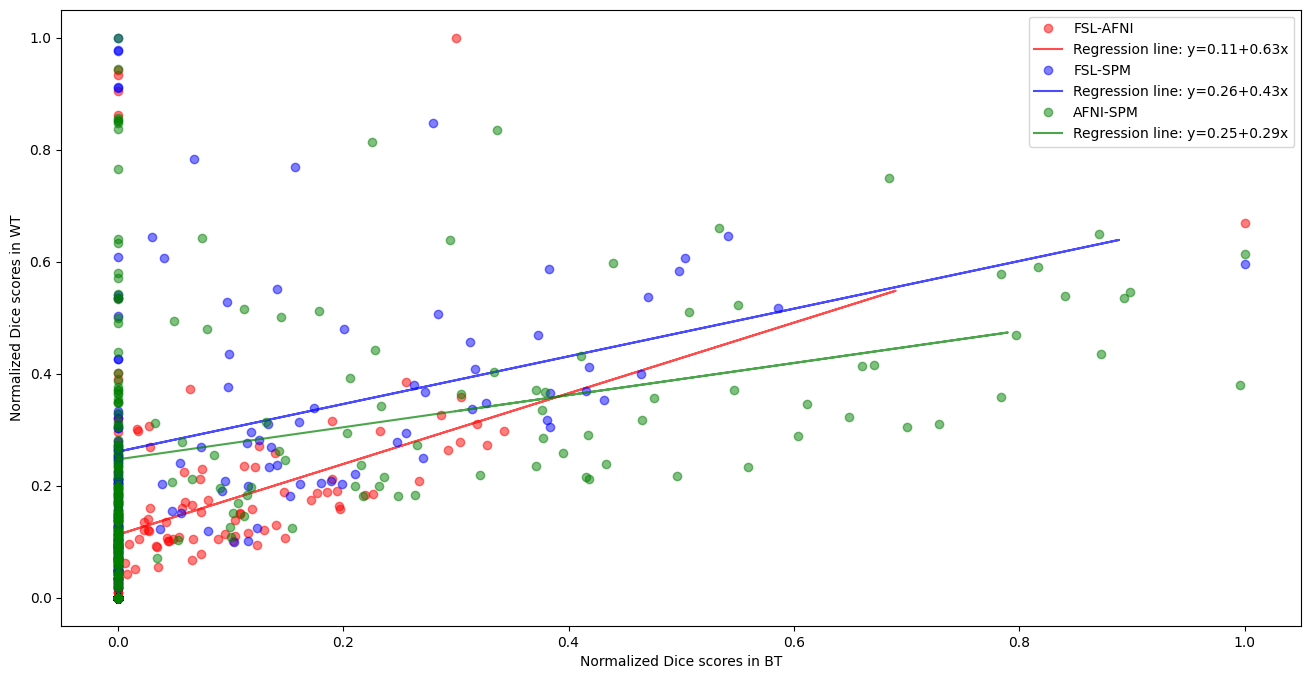
\includegraphics[width=\columnwidth]{figures/dices_corr.png}
    \caption{Correlation of Dice coefficients of activated regions between pair of tools and fuzzy samples
    from the thresholded T-statistics. Different pairs are illustrated in different colors. 
    Regions correspond to the 360 areas of cortical parcellation (HCP-MMP1.0)~\cite{glasser2016multi}.}
    \label{fig:dice-thresh}
    \end{minipage}}
  \end{figure}

%Fig 1
Comparisons of standard deviations between thresholded images in WT and BT
on MNI space are shown in Figure~\ref{fig:thresh-varmaps}.
While we observe substantial variations in BT (average std. dev. $\approx$ 1.5),
the order of magnitude of variations in WT is much lower (average std. dev. $\approx$ 0.5),
as was anticipated. However, numerical variability is still significant in WT results.
Moreover, we see the same order of magnitude in WT variations compared to BT variations
in some regions in the thresholded images.
For instance, we see parts of the frontal lobe in the sagittal plane for almost all pairs and the occipital lobe in the axial plane
for the pairs of \fslspm and \fslafni in Figure~\ref{fig:unthresh-varmaps}
that are closely simulated using the numerical perturbations. 


%%%%%%%%%% Var. of Thresh %%%%%%%%
\begin{figure*}[ht]
    \fbox{\begin{minipage}{\dimexpr \textwidth-2\fboxsep-2\fboxrule}
    \begin{subfigure}[t]{\textwidth}
      \centering
      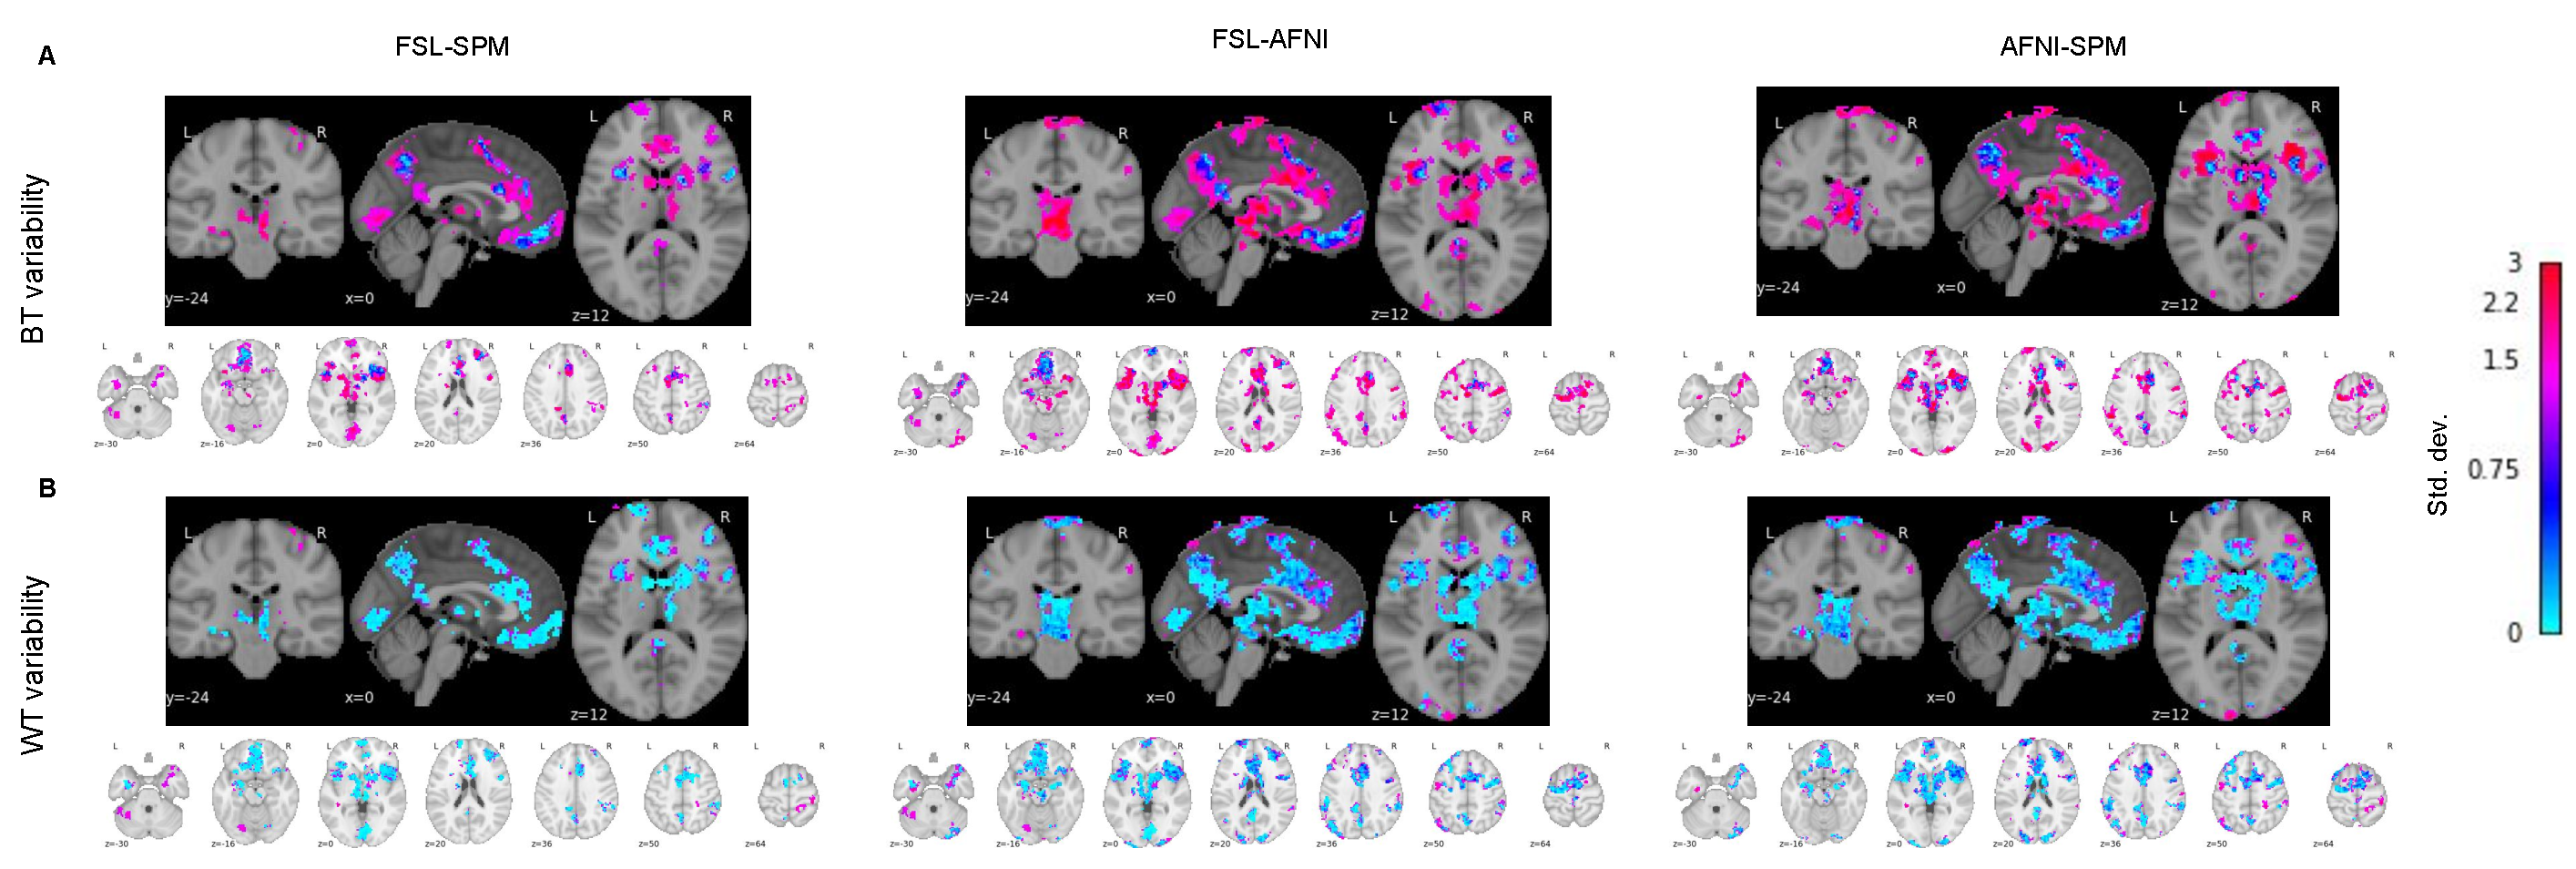
\includegraphics[width=\textwidth]{figures/bt-wt-thresh-std.pdf}
      %\caption{Standard deviation of thresholded t-statistics map on template surface}
      \label{fig:thresh-varmaps1}
    \end{subfigure}
    \hfill
    \begin{subfigure}[t]{\textwidth}
      \centering
      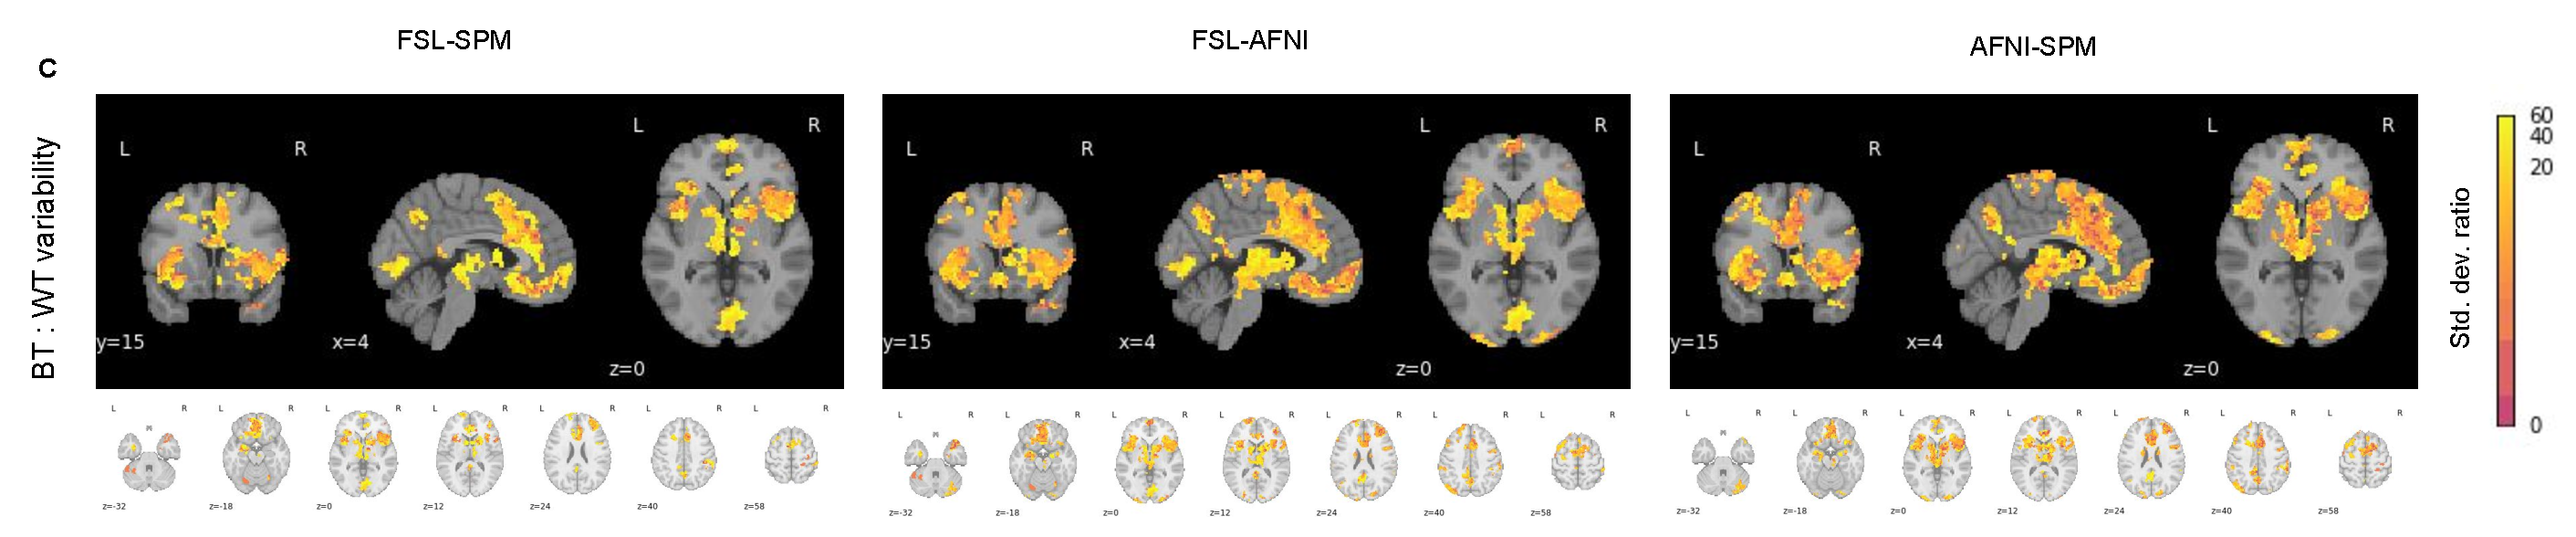
\includegraphics[width=\textwidth]{figures/ratio-thresh-std.pdf}
      %\caption{Standard deviation of thresholded t-statistics map on template surface}
      \label{fig:thresh-ratiomaps}
    \end{subfigure}
    \caption{Maps of standard deviation of thresholded T-statistics. First and second rows show
    maps on between-tool and within-tool results, respectively. Third row represents the ratio of differences
    in between and within tools.}
    % so that bright blue areas indicate more similar order of magnitude of variations in both conditions,
    %and vise versa for the darkder regions.}
    \label{fig:thresh-varmaps}
    \end{minipage}}
  \end{figure*}
  


% Fig2
In Figure~\ref{fig:dice-thresh}, we compare region-by-region Dice coefficients of
the group-level thresholded maps for all pairs of software packages in BT and WT.
This shows a linear correlation between Dice values in BT and WT,
which implies that the variability of activated voxels in both conditions is similar.
Also, small P-values across all three pairs, including 1x10e-10 for \fslafni, 6x10e-04 for \fslspm,
and 2x10e-05 for \afnispm, confirms this correlation of similarities.
The vertical line where the Dice score is zero in BT shows regions in the brain with no overlaps between activated voxels in BT but WT.
For instance, left/right `V1\_ROI' in \fslafni and \fslspm, and left/right `TGd\_ROI' in \afnispm results.
The regression line is computed over Dices where BT and WT are not zero.
% The average of Dice scores range from to 
% FSL-AFNI variations has the most similarity correlations which means that the results of these two tools are more \dots

% In response to the out of border activated voxels can say:
% This is likely due to the fact that SPM consistently had the smallest analysis mask out of the three packages,
% while FSL had the largest. Number of activated voxels prove this fact.



\subsection{Group-level unthresholded maps}

% Fig3
Figure~\ref{fig:unthresh-varmaps} shows the brain maps of standard deviations for group-level unthresholded T-statistics in WT and BT.
Results show a different magnitude of
the order of variations in WT and BT with standard deviation ranges from $\approx$ 0.12 to $\approx$ 0.5 on average, respectively.
The maps show regions in the brain where the magnitude of standard deviation is close to zero in WT but it exceeds 2.0 in BT,
such as the limbic and frontal lobes in the sagittal plane.
However, there are voxels with a significant correlation between WT and BT that are uniformly distributed across the brain maps.


%%%%%%%%%% Var. of Thresh %%%%%%%%
\begin{figure*}[b]
    \fbox{\begin{minipage}{\dimexpr \textwidth-2\fboxsep-2\fboxrule}
    \begin{subfigure}[t]{\textwidth}
      \centering
      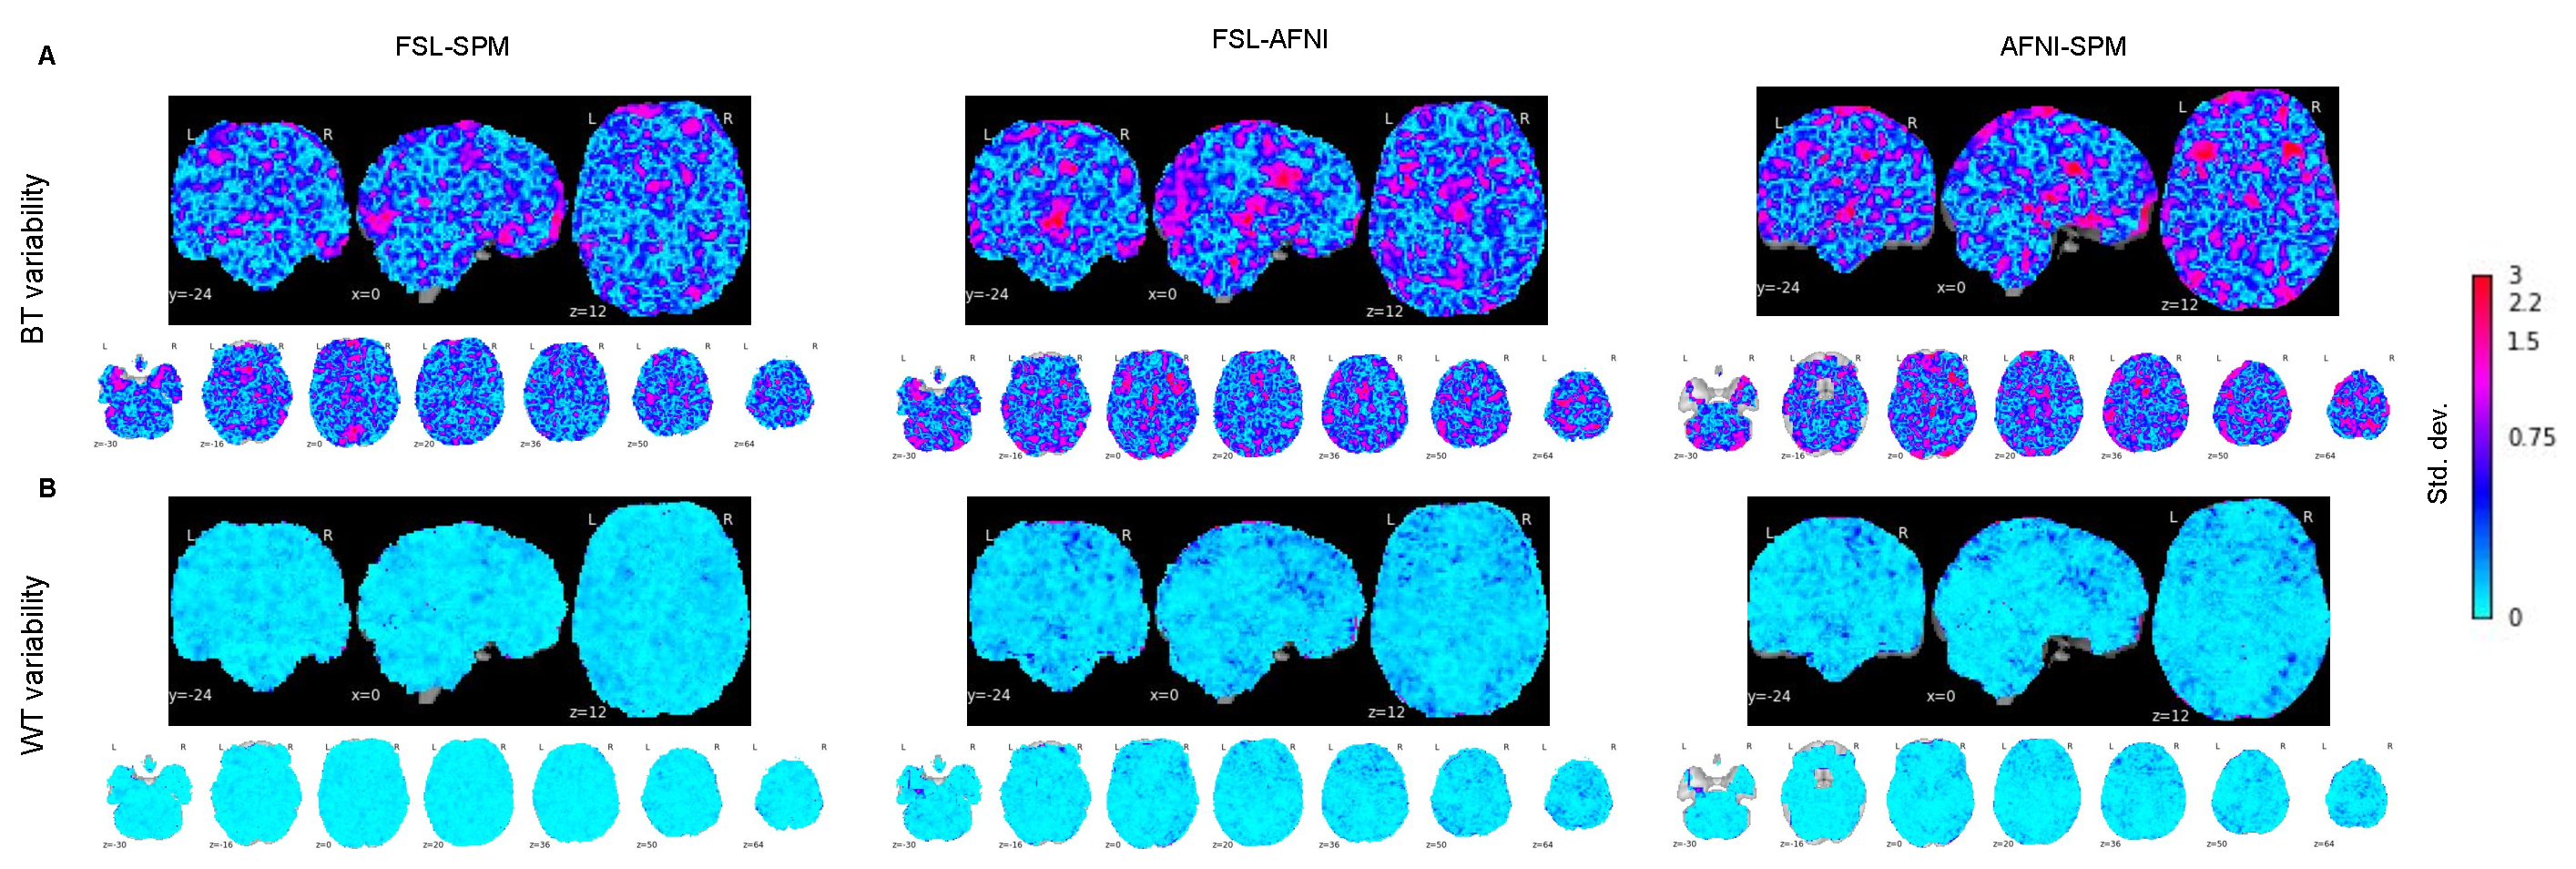
\includegraphics[width=\textwidth]{figures/bt-wt-unthresh-std.pdf}
      %\caption{Standard deviation of thresholded t-statistics map on template surface}
      \label{fig:unthresh-varmaps1}
    \end{subfigure}
    \hfill
    \begin{subfigure}[t]{\textwidth}
      \centering
      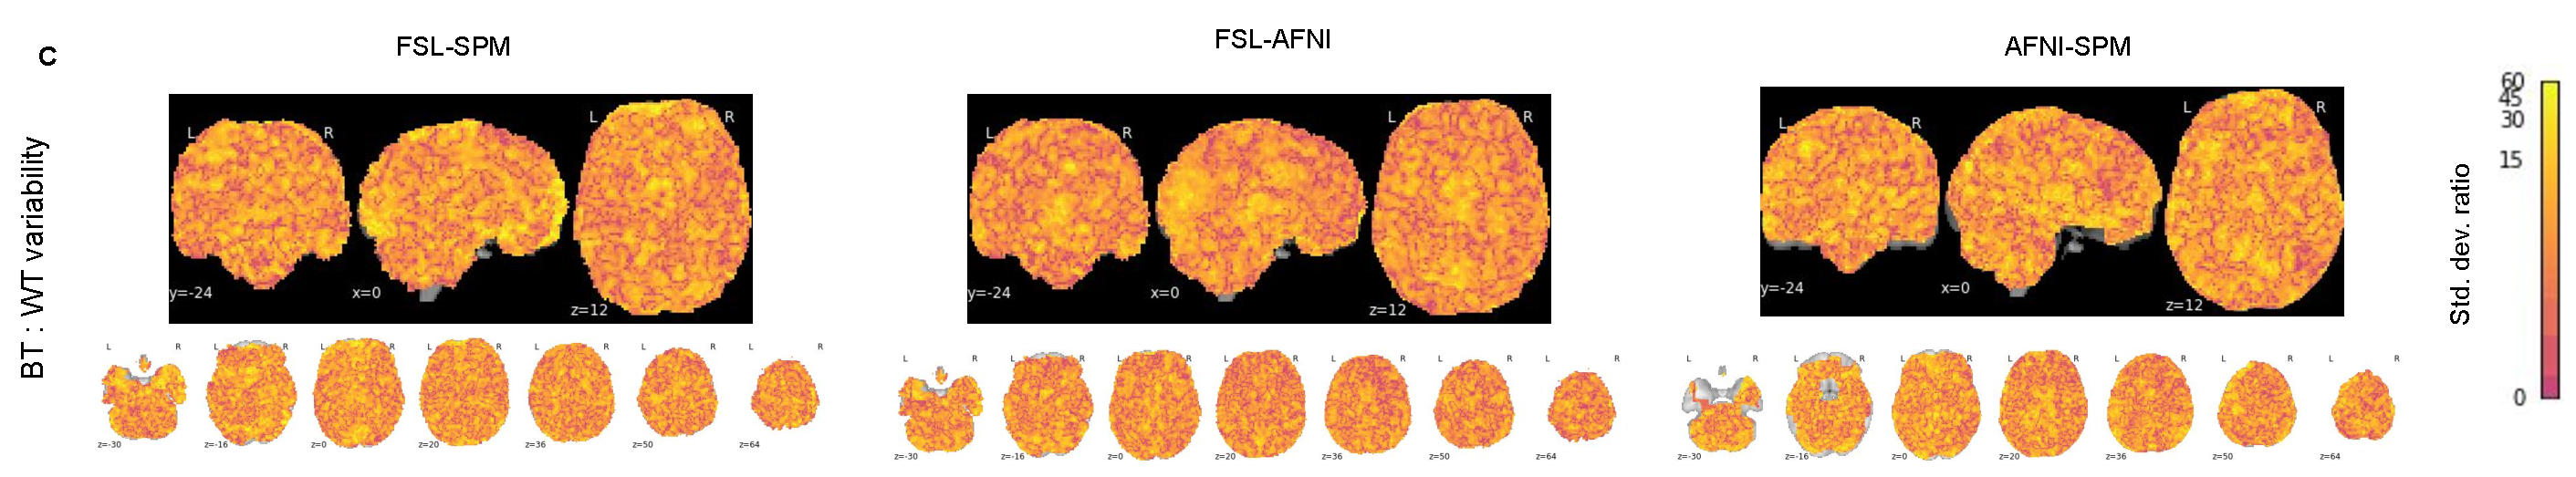
\includegraphics[width=\textwidth]{figures/ratio-unthresh-std.pdf}
      %\caption{Standard deviation of thresholded t-statistics map on template surface}
      \label{fig:unthresh-ratiomaps}
    \end{subfigure}
    \caption{Maps of standard deviation of unthresholded T-statistics. First and second rows show
    maps on between-tool and within-tool results, respectively. Third row represents the ratio of differences
    in between and within tools.}
    \label{fig:unthresh-varmaps}
    \end{minipage}}
  \end{figure*}
  

% Fig4
The scatter plot in Figure~\ref{fig:correlations} represents the correlation of standard deviation in WT and BT variability.
We found two major clusters, including the identity cluster that corresponds to the correlations
between BT and WT with the ratio of $0.5 < BT/WT < 1.5$,
and the upper cluster that shows voxels where BT $\approx$ 0.
The percentage of voxels included in the identity cluster is \%9.9 in \fslspm, \%17.3 in \fslafni, and \%13.8 in \afnispm,
and total voxels in the upper cluster are $\approx$ \%1.
The identity area is also represented on the MNI space in the second row in Figure~\ref{fig:correlations}.
This figure shows the spatial localization of the parts of the brain that BT variability is correlated with the numerical variability.
This refines the presented results in Figure~\ref{fig:unthresh-varmaps},
which indicates how correlation is uniformly distributed across the brain.
% Spatial localization of significant activation in the thresholded images also varied across software packages.
% Moreover, results show that pair of FSL-SPM has the least correlation of variability in within tool and between tool.
% This will implies that ... which can help for further investigations. 
  
  %%%%%%%%%% Corr. plot of tstats%%%%%%%%
  \begin{figure*}[b]
    \fbox{\begin{minipage}{\dimexpr \textwidth-2\fboxsep-2\fboxrule}
      \begin{subfigure}[t]{\textwidth}
        \centering
        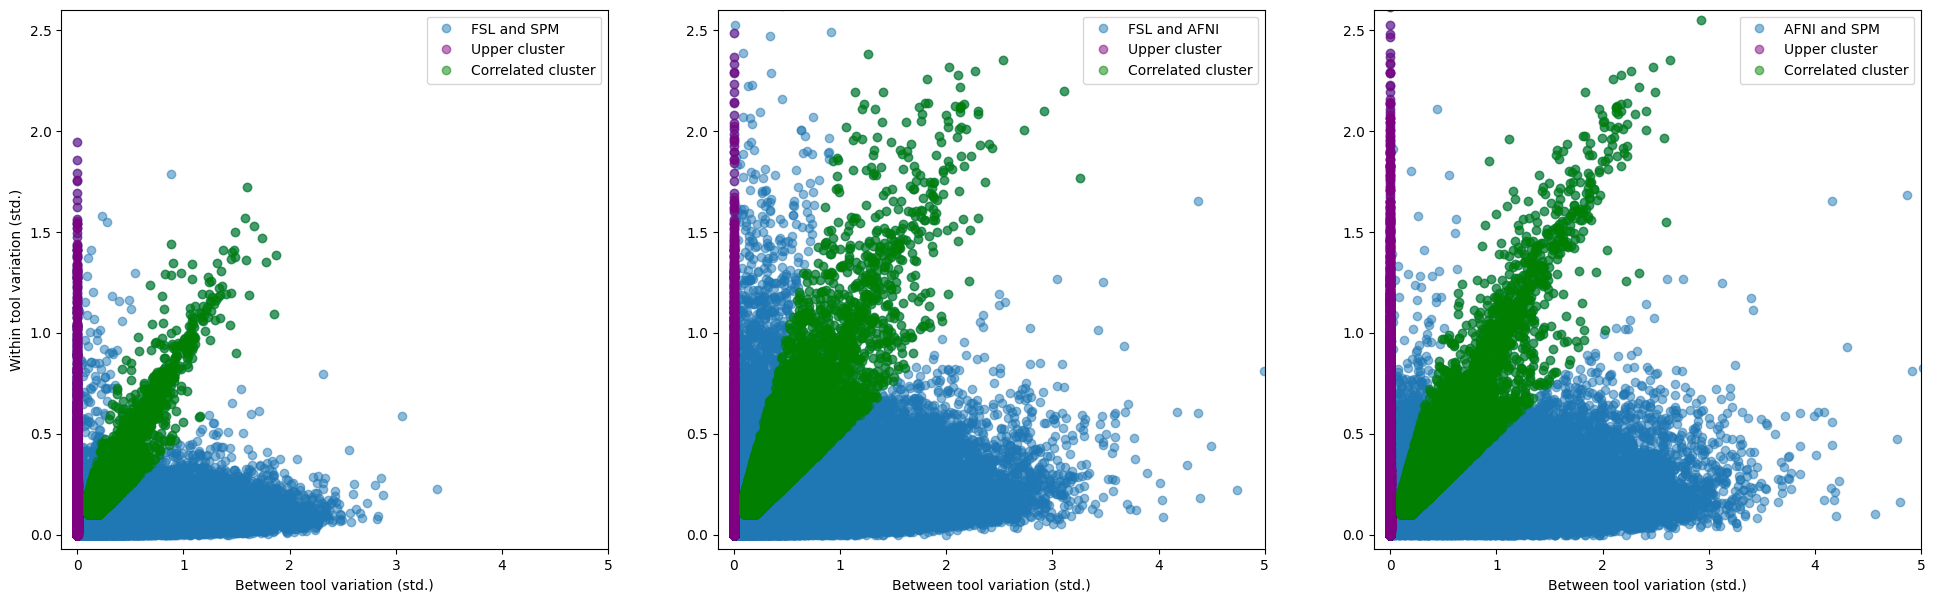
\includegraphics[width=\textwidth]{figures/std-corr-unthresh-plot.png}
        %\caption{Standard deviation of thresholded t-statistics map on template surface}
        \label{fig:unthresh-corrplot}
      \end{subfigure}
      \hfill
      \begin{subfigure}[t]{\textwidth}
        \centering
        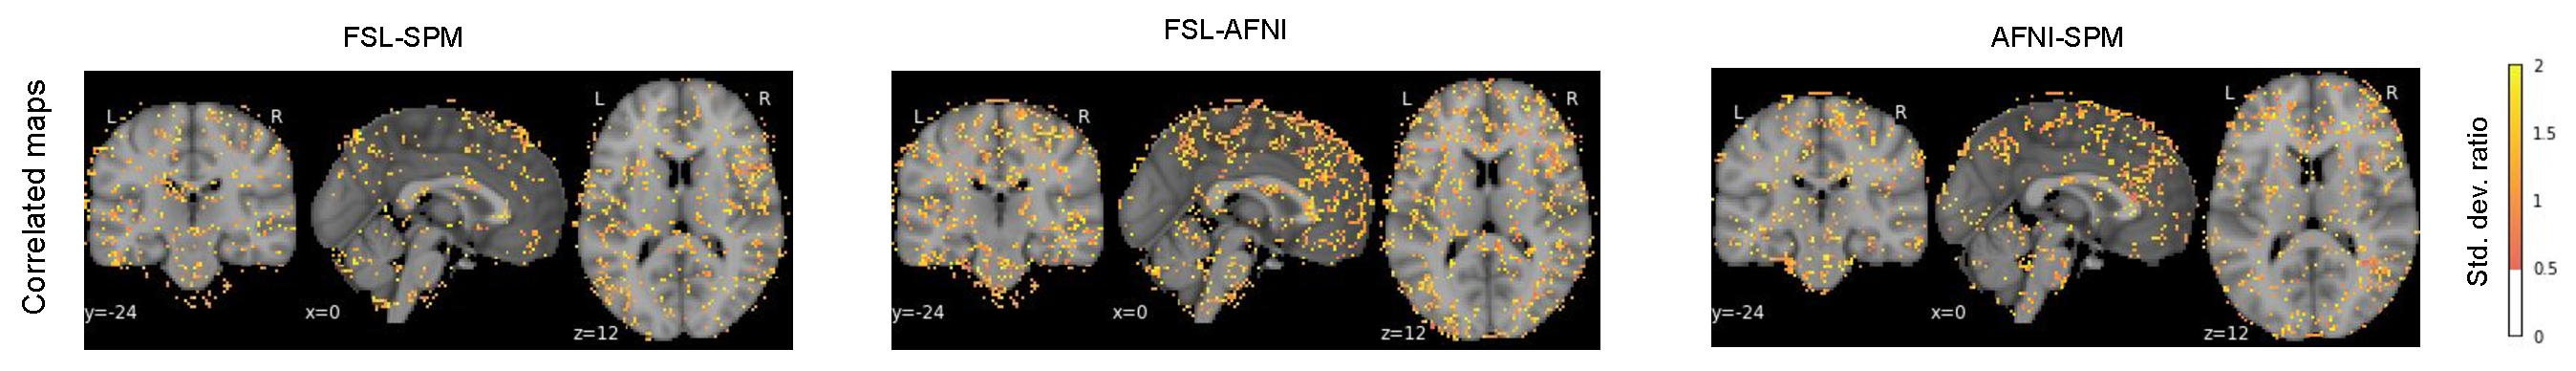
\includegraphics[width=\textwidth]{figures/corr-unthresh-std.pdf}
        %\caption{Standard deviation of thresholded t-statistics map on template surface}
        \label{fig:unthresh-corrmaps}
      \end{subfigure}
      \caption{Correlation of variability in between-tool and within-tool variations in unthresholded maps. First row plots the correlations
    voxel by voxel, which is highlighted with different colors for two major clusters including upper cluster (purple color) and
    correlated cluster (green color) which are mapped on the brain in the second row.}
    \label{fig:correlations}
    \end{minipage}}
  \end{figure*}
  
  

\section{Conclusion \& Discussion}


\begin{itemize}
    \item[$\bullet$ ] In this study, we represented the magnitude of differences in between tool and within tool results.
    We obtained more instability in BT compared to WT. Also we showed how between tool variations
    are correlated with numerical variability.
   
    \item[$\bullet$ ] Generally, we obtained more uncertainty on thresholded results, probably due to different thresholding
    methods used in different tools. This can raise further investigations on the thresholding techniques toward stability.
  
    \item[$\bullet$ ] Further studies can be evaluating the numerical stabilities within tool by focusing on the particular parts of 
    the pipeline that has been identified as the main sources of variations in~\cite{bowring2021isolating}.
    Also, we can invetigate the precision in WT variability that simulates mostly BT variability in the furure study.
    
\end{itemize}
  

\section{Acknowledgments} 


%%
%% The next two lines define the bibliography style to be used, and
%% the bibliography file.
\bibliographystyle{plain}
\bibliography{biblio}


\end{document}
\endinput
%%
%% End of file `sample-authordraft.tex'.
